\documentclass{article}
\usepackage[letterpaper, total={7in, 9.5in}]{geometry}
\usepackage{amsmath, amssymb}
\usepackage{tcolorbox}
\usepackage[dvipsnames]{xcolor}
\usepackage{ifthen}
\tcbuselibrary{listings,breakable}
\usepackage{float}
\usepackage{url}
\usepackage{enumitem}
\usepackage{hyperref} 

\usepackage{tikz}
\usetikzlibrary{shapes.geometric, arrows.meta, positioning}

%\usepackage{filecontents}      % lets you embed the CSV in the .tex file --- NOT NEEDED
\usepackage{pgfplots}          % main graphics package (loads TikZ)
\pgfplotsset{compat=1.18}      % pick the newest version you have

% ------------------------------------------------------------
%  Minimum preamble for PGFPlots box-plots from a CSV file
% ------------------------------------------------------------

% Extra PGFPlots libraries you need
\usepgfplotslibrary{statistics}    % ← provides \addplot+[boxplot]
\usepgfplotslibrary{colorbrewer}   % (optional) nicer default palettes

% Table handling (transpose, read CSV, etc.)
\usepackage{pgfplotstable}
% ------------------------------------------------------------

\title{Final Practice Problem Set}
\author{POL201.01 -- Introduction to Statistical Methods in Political Science}
\date{}

\begin{document}

\maketitle

\section{Midterm Topics}

% ------------------------------------------------------------------
%  INTRO TO DATA AND DESCRIPTIVE STATS — PRACTICE PROBLEMS  
% ------------------------------------------------------------------

\subsection{Understanding Data and Summary Statistics}
\textbf{Learning Goals}:
\begin{itemize}
    \item Identify whether a variable is categorical or numerical, and determine the level of measurement.
    \item Interpret summary statistics (mean, median, mode, range, IQR, standard deviation) in context.
    \item Use and interpret graphs: histograms, boxplots, bar plots, and mosaic plots.
    \item Describe the distribution of a variable in terms of shape, center, and spread.
\end{itemize}

\textbf{Questions}:
\begin{enumerate}
    \item \textbf{Variable Classification}  
    The table below lists several variables collected in a student survey. For each, classify the variable as \emph{categorical} or \emph{numerical}. If categorical, specify whether it is \emph{nominal} or \emph{ordinal}; if numerical, state whether it is \emph{discrete} or \emph{continuous}.

    \begin{center}
    \begin{tabular}{|l|l|}
    \hline
    \textbf{Variable} & \textbf{Sample Values} \\
    \hline
    Hours of sleep/night & 6, 7.5, 8, 5, 6.5 \\
    Major & Biology, Political Science, Econ \\
    Class standing & Freshman, Sophomore, Junior, Senior \\
    Number of roommates & 0, 1, 2, 2, 1 \\
    Opinion on new university logo & Strongly oppose to Strongly support (1--5 scale) \\
    \hline
    \end{tabular}
    \end{center}

    \item \textbf{Summary Statistics in Context} \\
    In a survey of 18 employees, the number of training sessions they attended last month was recorded as:
    \{1, 1, 1, 1, 1, 2, 2, 2, 2, 3, 3, 3, 4, 4, 5, 6, 6, 7\} \\
    Compute the sample mean and standard deviation. Then, interpret them in context.

    \item \textbf{Interpreting a Boxplot} \\
    A boxplot summarizes the distribution of hours studying or attending classes per week by a sample of college students.

\begin{center}
    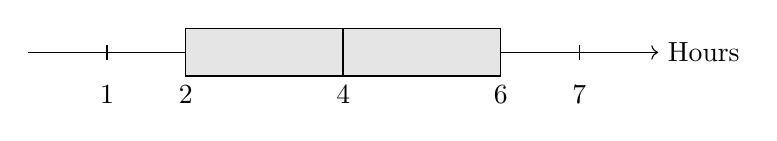
\begin{tikzpicture}
    % Axis
    \draw[->] (0,0) -- (8,0) node[anchor=west] {Hours};
    
    % Whiskers
    \draw (1,0.1) -- (1,-0.1); % Min
    \draw (7,0.1) -- (7,-0.1); % Max
    \draw (1,0) -- (2,0); % Left whisker
    \draw (6,0) -- (7,0); % Right whisker
    
    % Box
    \draw[fill=gray!20] (2,-0.3) rectangle (6,0.3);
    
    % Median
    \draw[thick] (4, -0.3) -- (4, 0.3);
    
    % Labels
    \node[below] at (1, -0.3) {1};
    \node[below] at (2, -0.3) {2};
    \node[below] at (4, -0.3) {4};
    \node[below] at (6, -0.3) {6};
    \node[below] at (7, -0.3) {7};
    \end{tikzpicture}
\end{center}


    \begin{itemize}
        \item Describe the shape, center, and spread of the distribution.
    \end{itemize}

    \item \textbf{Choosing the Right Graph} \\
    Recommend an appropriate graph type for each research question and justify your answer:
    \begin{enumerate}
        \item Is there a difference in political affiliation between men and women?
        \item What is the distribution of GPAs among students?
        \item Do students who live on campus differ in weekly study hours compared to off-campus students?
        \item What is the relationship between class attendance and final exam scores?
    \end{enumerate}

    \item \textbf{Describing a Distribution from a Histogram} \\
    A histogram displays the monthly income (in \$100s) of student workers.

    \begin{center}
    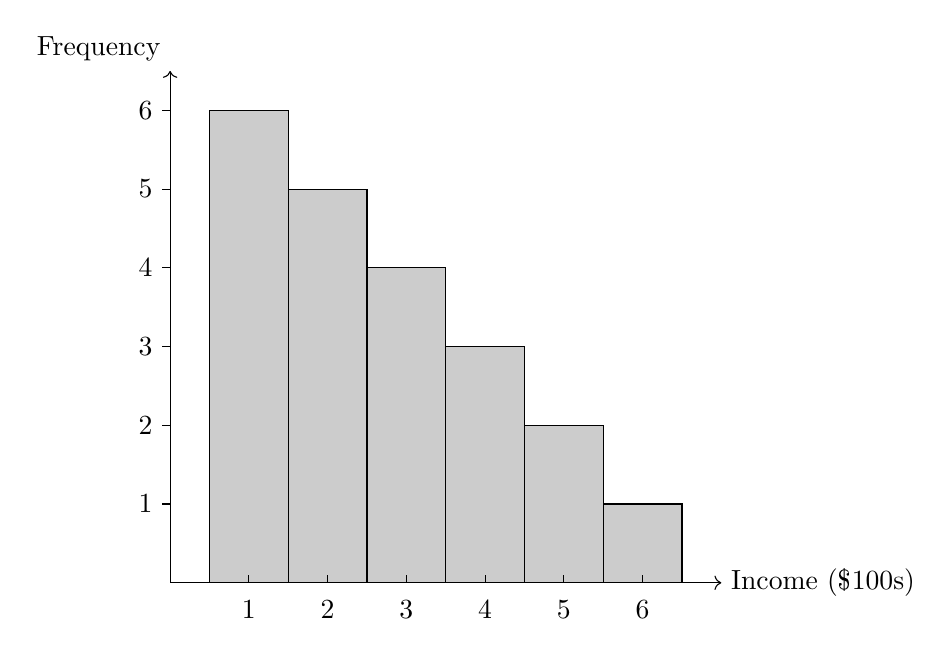
\begin{tikzpicture}
      % Axes
      \draw[->] (0,0) -- (7,0) node[anchor=west] {Income (\$100s)};
      \draw[->] (0,0) -- (0,6.5) node[anchor=south east] {Frequency};
    
      % Bars  (heights doubled)
      \draw[fill=gray!40] (0.5,0) rectangle (1.5,6);
      \draw[fill=gray!40] (1.5,0) rectangle (2.5,5);
      \draw[fill=gray!40] (2.5,0) rectangle (3.5,4);
      \draw[fill=gray!40] (3.5,0) rectangle (4.5,3);
      \draw[fill=gray!40] (4.5,0) rectangle (5.5,2);
      \draw[fill=gray!40] (5.5,0) rectangle (6.5,1);
    
      % x-axis ticks and labels
      \foreach \x in {1,...,6}{
        \draw (\x,0) -- (\x,0.1);
        \node[below] at (\x,-0.1) {\x};
      }
    
      % y-axis ticks and labels
      \foreach \y in {1,...,6}{
        \draw (0,\y) -- (-0.1,\y) node[left]{\y};
      }
    \end{tikzpicture}
    \end{center}
    

    \begin{enumerate}
        \item Compute the median. Compute the mean (use the weighted mean formula).
        \item Describe the shape, center, and spread of the distribution.
    \end{enumerate}

% --------------------------------------------------------------------------------------------
% ------------------------  Interpreting Two Box Plots  ------------------------
\item \textbf{Interpreting Two Box Plots} \\
The side-by-side box plots below summarise weekly study-hours for two groups of students.

\begin{center}
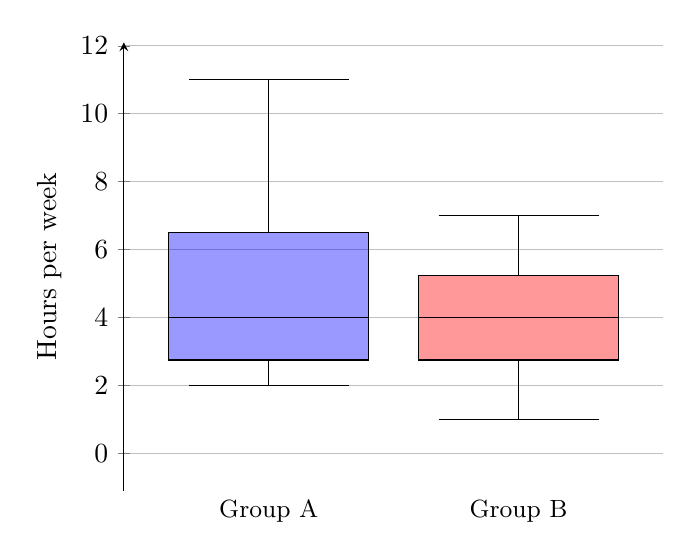
\begin{tikzpicture}
  % --- raw data ---------------------------------------------------------------
  % Each row is one group; PGFPlots will transpose so that every *column*
  % becomes a separate box plot.
  \begin{filecontents*}{twogroups.csv}
  2,2,3,4,4,6,8,11   % Group A (right-skewed) 
  1,2,3,4,4,5,6,7    % Group B (roughly symmetric)
  \end{filecontents*}

  % --- PGFPlots set-up --------------------------------------------------------
  \pgfplotstableread[col sep=comma]{twogroups.csv}\csvdata
  \pgfplotstabletranspose\datatransposed{\csvdata}   % rows → columns

  \begin{axis}[
      boxplot/draw direction         = y,
      x axis line style              = {opacity=0},
      axis x line*                   = bottom,
      axis y line                    = left,
      enlarge y limits,
      ymajorgrids,
      ymin                            = 0,
      ymax                            = 11,
      ylabel                          = {Hours per week},
      xtick                           = {1,2},
      xticklabels                     = {Group A, Group B},
      xticklabel style                = {align=center, font=\small},
      xtick style                     = {draw=none},  % hide tick line
  ]
    % left box: column 1 (Group A)
    \addplot+[boxplot, fill=blue,fill opacity=0.4,draw=black]  table[y index=1] {\datatransposed};
    
    % right box: column 2 (Group B)
    \addplot+[boxplot, fill=red,fill opacity=0.4,draw=black]   table[y index=2] {\datatransposed};
    
  \end{axis}
\end{tikzpicture}
\end{center}

\begin{itemize}
  \item Compare the two distributions in terms of \emph{shape, center, and spread}.  
        % Note in particular that both groups have the same median (4 hours) but Group A shows a much longer right tail, indicating greater variability and positive skewness.
\end{itemize}
% ----------------------------------------------------------------------------- 
\item \textbf{Interpreting a Scatter Plot with Two Groups} \\
The scatter plot below shows the relationship between Study Hours and GPA for two groups of students.

% --- Sample Data for Two Groups (x,y) pairs ---
\begin{filecontents*}{scatterdata.csv}
xA,yA,xB,yB
1,4,1,3
2,5,2,4
3,4,3,5
4,6,4,7
5,5,5,9
\end{filecontents*}


\begin{center}
\begin{tikzpicture}
\begin{axis}[
    xlabel = {Study Hours},
    ylabel = {GPA},
    legend style = {at={(0.5,-0.2)}, anchor=north, legend columns=2},
    width=10cm, height=7cm,
    grid=both,
    xmin=0, xmax=6,
    ymin=2, ymax=10
]
    % Group A
    \addplot+[
        only marks,
        mark=*,
        color=blue,
        fill=blue,
        fill opacity=0.5,
    ]
    table[x=xA, y=yA, col sep=comma] {scatterdata.csv};
    \addlegendentry{Group A}

    % Group B
    \addplot+[
        only marks,
        mark=*,
        color=red,
        fill=red,
        fill opacity=0.5,
    ]
    table[x=xB, y=yB, col sep=comma] {scatterdata.csv};
    \addlegendentry{Group B}

\end{axis}
\end{tikzpicture}
\end{center}

\textbf{Use the graph to answer the following:}
\begin{enumerate}
    \item Compute the \textbf{average GPA} and \textbf{average Study Hours} for each group. Interpret these averages in the context of student performance.
    
    \item Based on the scatter plot, describe the \textbf{association between Study Hours and GPA}. Is the association positive, negative, nonlinear, or are the variables independent? Support your answer using evidence from the plot.
    
    \item Which group shows a \textbf{stronger association} between Study Hours and GPA? Explain your reasoning.
\end{enumerate}


% ----------------------------------------------------------------------------------
\item \textbf{Understanding a Bimodal Distribution} \\
A histogram shows the number of hours students spent on screens in a single day. The sample includes 16 students.

\begin{center}
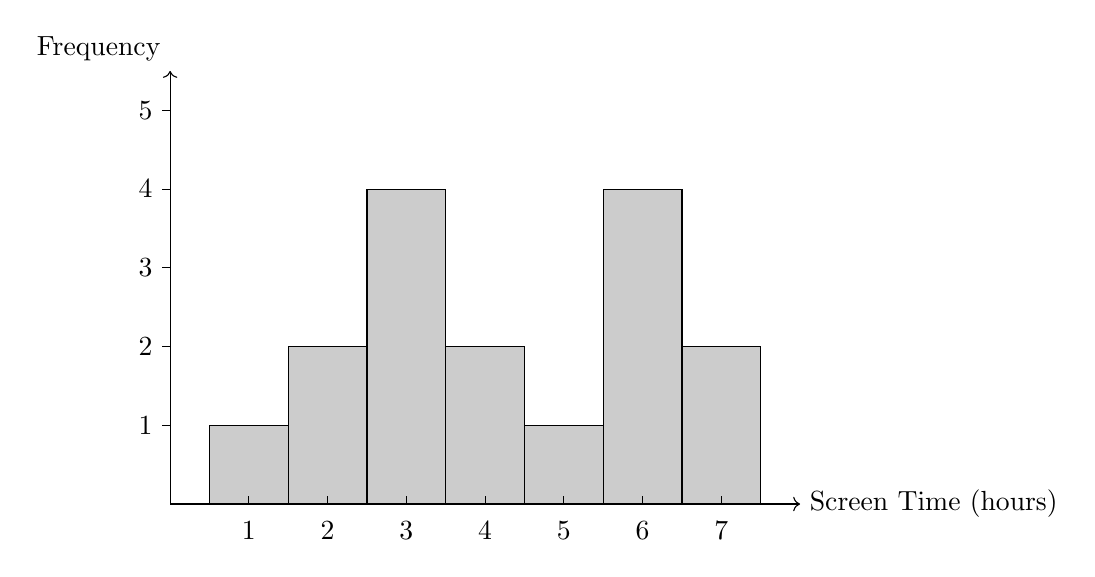
\begin{tikzpicture}
  % Axes
  \draw[->] (0,0) -- (8,0) node[anchor=west] {Screen Time (hours)};
  \draw[->] (0,0) -- (0,5.5) node[anchor=south east] {Frequency};

  % Bars
  \draw[fill=gray!40] (0.5,0) rectangle (1.5,1);
  \draw[fill=gray!40] (1.5,0) rectangle (2.5,2);
  \draw[fill=gray!40] (2.5,0) rectangle (3.5,4);
  \draw[fill=gray!40] (3.5,0) rectangle (4.5,2);
  \draw[fill=gray!40] (4.5,0) rectangle (5.5,1);
  \draw[fill=gray!40] (5.5,0) rectangle (6.5,4);
  \draw[fill=gray!40] (6.5,0) rectangle (7.5,2);

  % x-axis ticks and labels
  \foreach \x in {1,...,7}{
    \draw (\x,0) -- (\x,0.1);
    \node[below] at (\x,-0.1) {\x};
  }

  % y-axis ticks and labels
  \foreach \y in {1,...,5}{
    \draw (0,\y) -- (-0.1,\y) node[left]{\y};
  }
\end{tikzpicture}
\end{center}

\begin{enumerate}
    \item Describe the shape of the distribution. Is it symmetric, skewed, or something else?
    \item Identify the two modes and identify how many students fall into each.
    \item Compute the sample mean using a weighted average. Compare it to the modes: Is the mean a good summary here?
    \item If someone only reported the mean screen time from this data, what important features would be lost?
\end{enumerate}

\item \emph{Interpreting Affective Polarization from Summary Statistics (ANES 2020)} \\[0.5em]
In the 2020 American National Election Study (ANES), respondents were asked to rate their feelings toward major political parties using a \textbf{feeling thermometer} ranging from 0 (very cold/unfavorable) to 100 (very warm/favorable). This question is often used to study \emph{affective polarization}—how warmly or coldly people feel about the opposing political party.

The table below summarizes how Democrats and Republicans rated the \textbf{opposing party}:

\begin{center}
\begin{tabular}{|p{2.9cm}|c|c|c|c|c|c|c|c|c|}
\hline
\textbf{Group} & \textbf{Count} & \textbf{Mean} & \textbf{Median} & \textbf{Mode} & \textbf{Std. Dev.} & \textbf{Min} & \textbf{Q1} & \textbf{Q3} & \textbf{Max} \\
\hline
Democrats rating Republicans & 3,794 & 19.6 & 15.0 & 0.0 & 20.7 & 0.0 & 0.0 & 30.0 & 100.0 \\
Republicans rating Democrats & 3,407 & 17.7 & 15.0 & 0.0 & 20.9 & 0.0 & 0.0 & 30.0 & 100.0 \\
\hline
\end{tabular}
\end{center}

\begin{enumerate}
\item The mean for Democrats rating Republicans is 19.6, while for Republicans rating Democrats it’s 17.7, yet both medians are 15.0. What does the fact that the means differ but the medians are identical tell you about each distribution?

\item Both groups have Mode = 0.0 and Q1 = 0.0. What does that tell you about how many respondents gave the coldest possible rating?

\item In each case the mean exceeds the median, and the maximum is 100. Based on mean vs.\ median, which way are these distributions skewed, and why?

\item Q3 is 30.0 for both groups. What percentage of respondents rated the opposing party at 30 or higher?
\end{enumerate}




\end{enumerate}

% ------------------------------------------------------------------
%  PROBABILITY — PRACTICE PROBLEMS  (NO CALCULUS REQUIRED)
% ------------------------------------------------------------------

\subsection{Probability}
\textbf{Learning Goals}:
\begin{itemize}
    \item Define and apply concepts of sample space, events, disjoint and independent events.
    \item Use Venn diagrams and probability rules: addition, multiplication, complements.
    \item Calculate conditional probability and apply Bayes' theorem.
    \item Distinguish between discrete and continuous probability distributions.
\end{itemize}

\textbf{Questions}:
\begin{enumerate}
   \item A political analyst claims that support for a local tax increase (event A) and turnout in municipal elections (event B) are independent. Based on survey data, 50\% of residents support the tax increase, 40\% plan to vote, and 20\% both support the tax increase and plan to vote.  \\
    Which of the following conclusions is most appropriate?
    \begin{enumerate}
        \item[(A)] The analyst is correct; independence implies \( P(A \cap B) = 0.5 \times 0.4 = 0.20 \).
        \item[(B)] The events are not independent; independence would imply \( P(A \cap B) = 0.9 \).
        \item[(C)] The events are not independent; \( P(A \cap B) = 0.20 \) is too low compared to the expected value under independence.
        \item[(D)] There is not enough information to assess independence without knowing \( P(B|A) \).
    \end{enumerate}
    \item A public health study finds that 20\% of adults smoke. What is the probability that in a random sample of two adults, both smoke, assuming independence?
    \begin{enumerate}
        \item[(A)] 0.20  
        \item[(B)] 0.40  
        \item[(C)] 0.04  
        \item[(D)] 0.80  
    \end{enumerate}
    \item Suppose your friend flips a fair coin three times. What is the probability of getting exactly two heads? 
    \begin{enumerate}
        \item[(A)] 0.25  
        \item[(B)] 0.375  
        \item[(C)] 0.5  
        \item[(D)] 0.75  
    \end{enumerate}
\item An AI tool is designed to detect whether student essays are AI-generated. It analyzes a submitted essay and flags it as ``AI-generated" or ``Human-written." The tool has the following characteristics:
    \begin{itemize}
        \item If an essay is actually AI-generated, the tool correctly flags it 92\% of the time (true positive rate).
        \item If an essay is actually written by a human, the tool incorrectly flags it as AI-generated 8\% of the time (false positive rate).
        \item In a given semester, it is estimated that 35\% of submitted essays are AI-generated. 
    \end{itemize}
    If the AI tool flags an essay as "AI-generated," what is the probability that the essay was actually written by AI?
    \begin{enumerate}
        \item[(A)] 0.35 
        \item[(B)] 0.80 
        \item[(C)] 0.86 
        \item[(D)] 0.92
    \end{enumerate}
\end{enumerate}


% ------------------------------------------------------------------
%  RANDOM VARIABLES — PRACTICE PROBLEMS  (NO CALCULUS REQUIRED)
% ------------------------------------------------------------------
\subsection{Random Variables}
\textbf{Learning Goals}:
\begin{itemize}
    \item Define discrete and continuous random variables.
    \item Calculate expected value, variance, and standard deviation of discrete random variables.
    \item Use properties of linear combinations of random variables.
    \item Apply the binomial and normal distributions, and use standardization (z-scores).
\end{itemize}

\textbf{Questions}:

\begin{enumerate}
    %---------------------------------------------------------------
    \item \textbf{Standard Normal\,:  Z–scores}  \\
          An exam score $X$ is normally distributed with $\mu = 78$ and $\sigma = 6$.  
          \begin{enumerate}
              \item[(a)] Find the $Z$–score for a student who scored $85$.  
              \item[(b)] Using the CDF of the standard normal, compute $P(X \ge 85)$.  
          \end{enumerate}

    %---------------------------------------------------------------
    \item \textbf{Normal Approximation}  \\
          Let $\bar{X}$ be the mean of an i.i.d.\ sample of size $n=64$ taken from the distribution in Problem~1.  
          \begin{enumerate}
              \item[(a)] State the sampling distribution of $\bar{X}$ (mean and standard error).  
              \item[(b)] What is the probability $\Pr(\bar{X}\geq 80)$? Use the CLT and the standard normal CDF.  
              \item[(b)] What is the probability $\Pr(\bar{X}\leq 76)$? Use the CLT and the standard normal CDF.  
          \end{enumerate}

    %---------------------------------------------------------------
    \item \textbf{Bernoulli R.V.\ Basics}  \\
          A political ad in instagram is clicked with probability $p=0.12$.  Let $C$ be the indicator ($C=1$ if clicked, $0$ otherwise).  
          \begin{enumerate}
              \item[(a)] Write the Probability Mass Function (PMF) of $C$.  
              \item[(b)] Compute $\mathbb{E}[C]$ and $\operatorname{Var}(C)$.  
          \end{enumerate}

    %---------------------------------------------------------------
    \item \textbf{Binomial Probability}  \\
          An online campaign delivers $n=15$ independent \emph{ad impressions} to different users.  
          Each individual impression results in a click with probability $p = 0.12$, independently of all other impressions.  
          Let $Y$ be the random variable denoting the total number of clicks recorded in those 15 impressions, so that
          \[
          Y \sim \text{Binomial}\!\bigl(n=15,\,p=0.12\bigr).
          \]
          \begin{enumerate}
            \item[(a)] Compute the probability of observing \emph{exactly} three clicks, $\Pr(Y = 3)$.  
            \item[(b)] Compute the probability of observing \emph{at most} one click, $\Pr(Y \le 1)$.  
            \item[(c)] Compute the probability of observing \emph{more than} one click, $\Pr(Y > 1)$.  
          \end{enumerate}
    
    %---------------------------------------------------------------
    \item \textbf{Expected Value of a Discrete r.v.}  \\
          A game pays \$5, \$10, or \$25 with probabilities $0.60$, $0.30$, and $0.10$, respectively.  
          \begin{enumerate}
              \item[(a)] Let $W$ be the game's payout.  Compute $\mathbb{E}[W]$.  
              \item[(b)] Provide an intuitive interpretation of $\mathbb{E}[W]$ using plain language.
              \item[(c)] Compute $\operatorname{Var}(W)$.  
          \end{enumerate}

    %---------------------------------------------------------------
    \item \textbf{CDF Interpretation}  \\
          A discrete r.v.\ $Z$  can take on values $z \in \{0,1,2,3\}$ with pmf $p_Z(z=0)=0.1$, $p_Z(z=1)=0.4$, $p_Z(z=2)=0.3$, $p_Z(z=3)=0.2$.  
          \begin{enumerate}
              \item[(a)] Write the cumulative distribution function $F_Z(z)$.  
              \item[(b)] Use $F_Z$ to compute $\Pr(1<Z\le 3)$.  
          \end{enumerate}

    %---------------------------------------------------------------
    \item \textbf{A Basic Linear Combination\,—\,Mean and Variance - Part I}  \\
        Let \( X_1, X_2, \dots, X_n \) be independent and identically distributed (i.i.d.) random variables with mean \( \mu \) and variance \( \sigma^2 \). Suppose two distinct observations \( i \ne j \) are selected at random, and we define their difference as \( D = X_j - X_i \).  
        
        Derive expressions for \( \mathbb{E}[D] \) and \( \operatorname{Var}(D) \) in terms of \( \mu \) and \( \sigma^2 \).

%---------------------------------------------------------------
\item \textbf{A Basic Linear Combination\,—\,Mean and Variance - Part II}  \\
    Let \( X_1, X_2, \dots, X_n \) be independent and identically distributed (i.i.d.) random variables with mean \( \mu \) and variance \( \sigma^2 \). Suppose two distinct observations \( i \ne j \) are selected at random, and we define their midpoint as \( M = \frac{1}{2}(X_i + X_j) \).  
    
    Derive expressions for \( \mathbb{E}[M] \) and \( \operatorname{Var}(M) \) in terms of \( \mu \) and \( \sigma^2 \).


    %---------------------------------------------------------------
    \item \textbf{Distribution of a Sample Proportion}  \\
          In a survey $n=200$ voters are asked if they favor a policy ($1=$yes, $0=$no).  Let $\hat{p}$ be the sample proportion favouring it.  
          Suppose the true population proportion is $p=0.48$.  
          \begin{enumerate}
              \item[(a)] Give the mean and standard error of $\hat{p}$.  
              \item[(b)] Approximate $\Pr(\hat{p}\ge 0.55)$ using the normal approximation to the binomial and a $Z$–score.  
          \end{enumerate}

\end{enumerate}


\section{Post-Midterm Topics}

% ------------------------------------------------------------------
%  ESTIMATORS AND SAMPLING DISTRIBUTIONS
% ------------------------------------------------------------------
\subsection{Estimators and Sampling Distributions}
\textbf{Learning Goals}:
\begin{itemize}
    \item Differentiate between population parameters and sample estimators, and define the properties of unbiasedness, consistency, and efficiency.
    \item Describe the concept of a sampling distribution and explain its role in statistical inference.
    \item Calculate and interpret the standard error of sample estimators, including how it changes with sample size.
\end{itemize}

\textbf{Questions}:

Below are six questions that highlight the role of \emph{estimators} in making inferences about populations based on sample data. Each question is followed by four answer options, with only one correct choice. These are purely conceptual and do not require numerical calculations.

\begin{enumerate}
    \item \textbf{Which statement captures the primary goal of using an \emph{estimator} in statistics?}
        \begin{enumerate}
        \item[(A)] To remove randomness from the observed data.
        \item[(B)] To generate a single numerical value that matches the population parameter.
        \item[(C)] To forecast the probability for a range of values for the population using only observed frequencies.
        \item[(D)] To use sample data to approximate a population quantity and acknowledge possible sampling variation.
        \end{enumerate}
    \item \textbf{Consider the following statement:} \newline 
        \emph{``Since any estimate is one possible result from a single sample, we shouldn’t trust it as there is no way to know how representative it is.”} \newline 
        Which of the following best evaluates the truth and reasoning of this statement?
        \begin{enumerate}
        \item[(A)] The statement is \textbf{True}, because estimates are inherently unreliable and can’t be evaluated.
        \item[(B)] The statement is \textbf{True}, because without knowing the population, we have no grounds to assess an estimate’s accuracy.
        \item[(C)] The statement is \textbf{False}, because although estimates come from samples, we can quantify their uncertainty using sampling distributions.
        \item[(D)] The statement is \textbf{False}, because most sample estimates exactly match the population value in practice.
        \end{enumerate}
    \item \textbf{Suppose a survey estimates that 52\% of participants favor a new policy. From an inference standpoint, what is the key consideration for this estimated proportion?}
        \begin{enumerate}
        \item[(A)] Whether it is guaranteed to match the exact population proportion of 52\%.
        \item[(B)] How well it accounts for the fact that the sample proportion can vary due to random sampling.
        \item[(C)] Whether 52\% is larger than every other statistic we might collect.
        \item[(D)] How to reduce the sample size so the estimate becomes simpler to calculate.
        \end{enumerate} 
    \item  \textbf{3. When we call $X$ a \emph{random variable} that underlies our observed data points $x_i$, what do we mean in the context of making estimates?}
        \begin{enumerate}
        \item[(A)] We treat each $x_i$ as a random draw from a distribution, helping us formalize the behavior of an estimator using $x_i$.
        \item[(B)] $X$ is a fixed quantity that never changes.
        \item[(C)] $X$ is always continuous, and cannot represent discrete outcomes.
        \item[(D)] Each observed $x_i$ is unrelated to any population measure.
        \end{enumerate}
    \item  \textbf{The \emph{expected value} of a random variable $X$ (often denoted $E[X]$) is conceptually important because:}
        \begin{enumerate}
        \item[(A)] It identifies the most likely single outcome that $X$ can take.
        \item[(B)] It is a theoretical value describing the long-run average, which we often attempt to estimate using sample means.
        \item[(C)] It is calculated by identifying the midpoint between the highest and lowest values of $X$.
        \item[(D)] It remains purely symbolic and has no connection to real-world data or estimators.
        \end{enumerate}
    \item  \textbf{In describing an \emph{estimator} for a population quantity, why do we talk about the \emph{distribution} of sample outcomes?}
        \begin{enumerate}
        \item[(A)] Because the distribution allows us to determine the most common value of the estimator and treat it as the population parameter.
        \item[(B)] Because knowing the full distribution ensures that a single sample estimate will be unbiased.
        \item[(C)] Because sample distributions always approximate the population distribution, regardless of sample size.
        \item[(D)] Because it helps us understand how an estimator (like a sample mean or proportion) might vary across repeated samples.
        \end{enumerate}
    \item  \textbf{Which statement best summarizes how \emph{modeling assumptions} aid in interpreting an estimator's result?}
        \begin{enumerate}
        \item[(A)] They ensure that the estimator will converge exactly to the population parameter, regardless of sample size.
        \item[(B)] They justify treating the sample statistic as equal to the population value if the data fit the model well.
        \item[(C)] They allow us to use theoretical tools (like probability distributions) to quantify sampling uncertainty, even when we only have one observed sample.
        \item[(D)] They make it possible to generalize the estimator’s result to any population, regardless of how the data were collected.
        \end{enumerate}
\end{enumerate}

% ------------------------------------------------------------------
%  INFERENCE PROPORTIONS
% ------------------------------------------------------------------
\subsection{Inference for One and Two Proportions}
\textbf{Learning Goals}:
\begin{itemize}
    \item Construct and interpret confidence intervals for a population proportion.
    \item Conduct hypothesis tests for a single population proportion.
    \item Check conditions for using the normal approximation (CLT conditions).
    \item Construct and interpret confidence intervals for the difference between two proportions.
    \item Conduct hypothesis tests comparing two population proportions.
    \item Calculate and interpret pooled and unpooled standard errors.
\end{itemize}

\textbf{Questions}:
\begin{enumerate}
%-------------------------------------------------------------
\item  \emph{Framing the responsibility} \\
      A YouGov survey conducted on April 7, 2025, asked $n = 4{,}610$ U.S.\ adults how responsible they believe President Donald Trump is for the stock market. Of those surveyed, $43\%$ said he is \emph{very responsible}, and an additional $24\%$ said he is \emph{somewhat responsible}.\footnote{\textbf{Source:} YouGov. “How responsible, or not responsible, is President Donald Trump for the stock market?” April 7, 2025. Retrieved from \href{https://today.yougov.com/topics/politics/survey-results/daily/2025/04/07/6be5c/3}{today.yougov.com}}
      \begin{enumerate}[label=(\alph*)]
         \item Compute a 95\% confidence interval for the proportion of U.S.\ adults who say Trump is \textbf{very responsible}.  
         \item Compute a 95\% confidence interval for the proportion who say he is \textbf{at least somewhat responsible} (i.e., \emph{very} or \emph{somewhat} responsible).  
         \item Some media outlets claim “a majority of Americans believe Trump is responsible for the stock market.” Based on your intervals, evaluate whether that claim is supported. How does the conclusion differ depending on which group (very vs. at least somewhat) is analyzed?
      \end{enumerate}

%-------------------------------------------------------------
\item \emph{A super majority support?} \\ A February 2025 national survey by YouGov of $n=4{,}334$ U.S.\ adults found that $2{,}904$ respondents 
      said they would support amending the Constitution to set a maximum age (e.g.\ 75) for federal elected officials.\footnote{\textbf{Source:} YouGov. “Do you support or oppose setting a maximum age for elected officials?” Daily Question, February 21, 2025. Retrieved from \url{https://today.yougov.com/topics/politics/survey-results/daily/2025/02/21/a75c8/3}}
      \begin{enumerate}[label=(\alph*)]
         \item Compute a 95\% confidence interval for the true proportion of U.S.\ adults who favor the amendment.  
         \item Does the interval include the 60\% mark commonly cited as a “super‑majority” threshold?  Interpret.  
         \item A group of politicians claims “well over two‑thirds” of voters favour the amendment.  Test this claim at $\alpha=0.05$.
      \end{enumerate}
      
%-------------------------------------------------------------
\item \emph{Is there a gender gap in belief about AI emotions?} \\
      A June 2022 YouGov poll asked $n = 2{,}434$ U.S.\ adults whether they believe computers will ever experience feelings and emotions. Among male respondents, $26\%$ said “yes”; among female respondents, $16\%$ said “yes.” Assume the sample was evenly split between men and women.\footnote{\textbf{Source:} YouGov. “Do you think computers will ever experience feelings and emotions?” June 14, 2022. Retrieved from \href{https://today.yougov.com/}{today.yougov.com}}

      \begin{enumerate}[label=(\alph*)]
         \item State appropriate null and alternative hypotheses to test whether men and women differ in belief about computers experiencing emotions.
         \item Conduct a two-proportion $z$-test at the $\alpha = 0.05$ significance level.
         \item Interpret the result in context. Is there convincing statistical evidence of a gender gap in this belief? How large is the difference, practically speaking?
      \end{enumerate}
      
%-------------------------------------------------------------
\item  \emph{Remote vs.\ on‑campus learning outcomes.} \\
      Among 180 students who took a course fully online, 139 passed the final exam;  
      of 150 similar students who took the same course on campus, 123 passed.
      \begin{enumerate}[label=(\alph*)]
          \item Compute the pooled standard error and the $z$ statistic for testing equality of pass rates.  
          \item At $\alpha=0.10$, do the data provide evidence that the on‑campus format yields a higher pass rate? 
      \end{enumerate}

%-------------------------------------------------------------
\item  \emph{Vaccine acceptance across age groups.} \\
      A survey of 700 adults aged 18–34 finds 427 willing to take a new booster, while
      536 of 860 adults aged 55 + say the same.
      \begin{enumerate}[label=(\alph*)]
          \item Give a 99\% confidence interval for the difference in acceptance proportions (younger minus older).  
          \item Interpret the interval in context—be explicit about direction and magnitude.  
      \end{enumerate}

%-------------------------------------------------------------
\item  \emph{Margin of Error and Design Effects in Public Opinion Polls.}\\
    Pollsters frequently report the margin of error (MoE) as a way of conveying the uncertainty around estimated population proportions based on a sample. For binary outcomes (e.g., support vs. not support), the MoE is tied to the standard error (SE) of the sample proportion, which under simple random sampling (SRS) is given by:
    \[
    SE_{\text{SRS}} = \sqrt{\frac{p(1 - p)}{n}}
    \]
    In applied practice, pollsters often use $p_0 = 0.5$ when reporting MoE, as this value maximizes the standard error and hence yields a conservative (i.e., maximal) margin of error. Thus, the MoE under SRS becomes:
    \[
    MoE_{\text{SRS}} = z^* \cdot SE_{\text{SRS}}
    \]
    However, real-world survey designs frequently deviate from SRS by incorporating elements like stratification or clustering. These design features tend to increase the variance of the estimate relative to an SRS, and this inflation is captured using the \textbf{design effect (DEFF)} coefficient:
    \[
    SE_{\text{real}} = \sqrt{\text{DEFF}} \cdot SE_{\text{SRS}}
    \]
    The design effect quantifies how much the actual sampling variance exceeds the variance expected under SRS.
    
    \noindent\textbf{Question Statement and Problems:} \\
    An \emph{Economist/YouGov} poll conducted June 24–26, 2018, reports results from a sample of $n = 1{,}500$ U.S.\ adults, with a stated margin of error of $\pm 3.1\%$.%
    \footnote{\textbf{Source:} \emph{The Economist}/YouGov Poll, June 24–26, 2018. Retrieved from \url{https://today.yougov.com/sports/articles/21100-not-much-world-cup-excitement-us}}
    
    \begin{enumerate}
        \item[(a)] Assume $p_0 = 0.5$ as a conservative benchmark of the population proportion. Compute the standard error under the SRS assumption, $SE_{\text{SRS}}$.
    
        \item[(b)] Using your result from (a), express the theoretical margin of error under the SRS assumption, $MoE_{\text{SRS}}$, in terms of a generic critical value $z^*$.

        \item[(c)] Write both \( \text{MoE}_{\text{real}} \) and \( \text{MoE}_{\text{SRS}} \) as \( z^* \cdot SE \), and substitute \( SE_{\text{real}} = \sqrt{\text{DEFF}} \cdot SE_{\text{SRS}} \) into the expression for \( \text{MoE}_{\text{real}} \). Then form the ratio \( \frac{\text{MoE}_{\text{real}}}{\text{MoE}_{\text{SRS}}} \), cancel common terms, and show that it equals \( \sqrt{\text{DEFF}} \). Finally, square both sides and use your answer from part (b) to derive a formula for \( \text{DEFF} \) as a function of $\text{MoE}_{\text{real}}$, $z^*$, and $\text{SE}_{\text{SRS}}$.

        \item[(d)] Assume that most pollsters report a margin of error using a 95\% confidence level, so that \( z^* = 1.96 \). \\
        Use this value along with your standard error from part (a) to compute \( \text{MoE}_{\text{SRS}} = z^* \cdot SE_{\text{SRS}} \). \\
        Then, apply the formula you derived in part (c) to calculate the design effect (\( \text{DEFF} \)) using the reported \( \text{MoE}_{\text{real}} = 0.031 \).

        \item[(e)] Interpret the design effect value you calculated in part (d) using plain language. How many times larger is the actual standard error ($SE_{\text{real}}$) compared to the theoretical standard error under simple random sampling ($SE_{\text{SRS}}$)? What does this tell you about the additional level of uncertainty introduced by the real-world survey design?

    \end{enumerate}

%-------------------------------------------------------------
\item  \emph{Margin of What, Exactly? — Part II}. \\
    In the previous question, you explored how the margin of error (MoE) reflects the uncertainty around sample estimates under both simple random sampling and more realistic survey designs, and how it connects to the standard error and design effect (DEFF). You also worked with an example from an Economist/YouGov poll conducted June 24–26, 2018, which reported a margin of error of $\pm 3.1\%$ for a sample of $n = 1{,}500$ U.S. adults.
    
    In this part, we shift from the mathematical mechanics of margin of error to its practical interpretation. Poll results are often cited in the media or used to inform decision-making, but the reported MoE applies under specific assumptions—and not uniformly to all figures in the report.
    
    \begin{enumerate}[label=(\alph*)]
    \item One question found that 52\% of respondents said they do not personally know anyone who is an illegal immigrant. How should we interpret the margin of error in this context? What interval captures the plausible range for this percentage in the U.S. adult population at the 95\% confidence level? \footnote{Remember to account for the found design effect ($DEFF$) on the $SE(\hat{p})$ in the previous question, when you compute the $SE$ for $\hat{p}=0.52$.}
    \item Does the reported margin of error apply to all values in the poll (e.g., subgroups like “men under 30”)? Why or why not?
    \item What margin of error do you expect for subgroups in the sample with few respondents compared to the reported margin of error? A larger, similar, or smaller one? Why?
    \item Suppose the margin of error were larger—say, $\pm 5\%$. What could cause that, and how would it affect our conclusions about close issues or public opinion trends?
    \item Why is the margin of error not the only source of uncertainty in interpreting poll results?
    \end{enumerate}

\item  \emph{Partisan optimism about AI?} \\
      A YouGov survey conducted April 23–25, 2025, asked $n = 1{,099}$ U.S.\ adult citizens about the effect of artificial intelligence (AI) on society. Among Democrats ($n = 351$), $12\%$ described the effects as “very positive” and $26\%$ as “somewhat positive.” Among Republicans ($n = 293$), the corresponding figures were $7\%$ and $39\%$, respectively.\footnote{\textbf{Source:} YouGov Survey: AI Uses, April 23–25, 2025. Retrieved from \href{https://d3nkl3psvxxpe9.cloudfront.net/documents/AI_Uses_poll_results.pdf}{YouGov Survey: AI Uses}}

      \begin{enumerate}[label=(\alph*)]
         \item Combine the relevant categories and compute the proportion of each group (Democrats and Republicans) that sees AI’s effect as at least somewhat positive.
         \item Conduct a two-proportion $z$-test at the $\alpha = 0.05$ level to test whether there is a significant partisan difference in positive views of AI.
         \item Interpret your result in context. Is there statistical evidence of a difference in optimism about AI across party lines?
         \item Suppose a news headline claims, “Republicans are significantly more optimistic about AI than Democrats.” Do your results support this claim? What’s the difference between statistical and rhetorical significance?
      \end{enumerate}

\end{enumerate}

% ------------------------------------------------------------------
%  INFERENCE MEANS - LARGE SAMPLES
% ------------------------------------------------------------------

\subsection{Inference for One and Two Means (Large Sample)}
\textbf{Learning Goals}:
\begin{itemize}
    \item Construct and interpret confidence intervals for one or two population means using large-sample z-procedures.
    \item Perform hypothesis testing for one or two means when sample sizes are large.
    \item Check CLT-based conditions for inference.
\end{itemize}

\textbf{Questions}:
\begin{enumerate} % ---------------------------

\item \textbf{An urban planning problem} \\
Suffolk County plans to redevelop a large brownfield site into \(\mathbf{1\,200}\) single‑family homes.  
Suppose the county’s \emph{Comprehensive Plan 2015} assumed an average of \(\boldsymbol{\mu_0 = 2.8}\) persons per household when sizing roads, utilities, and schools.  
To check whether this benchmark is still valid, planners survey a simple random sample of \(n = 1\,000\) nearby households and record the number of people living in each. The following are the results of this survey.\footnote{\textbf{Sources:} U.S. Census Bureau. “Selected Social Characteristics in the United States,” ACS 1-Year Estimates (Table DP02), Suffolk County, NY, 2023. \href{https://data.census.gov/table/ACSDP1Y2023.DP02?q=DP02&g=050XX00US36103&d=ACS+1-Year+Estimates+Data+Profiles}{data.census.gov}}
\[
\bar{x}=3.00 \quad\text{persons}\qquad
s = 1.25 \quad\text{persons}
\]
\begin{enumerate}[label=(\alph*)]
  \item Construct a 99\% confidence interval for the true mean household size \(\mu\). Interpret the interval both in technical terms and in plain language.
  \item Using \(\alpha = 0.01\), test the hypothesis that the average household size still equals or is below the old planning figure:  
        \[
           H_0\!: \mu \le 2.8
           \quad\text{vs.}\quad
           H_a\!: \mu > 2.8.
        \]
  \item If the development proceeds, give a plausible \emph{range} for the additional population the county should plan for (low and high ends) based on your interval in part (a).
  \item County officials plan to use your estimate of total population to help size a new K–8 school for the development. In plain language, explain how sampling uncertainty in household size affects their decision. Why is it important to consider a range of values rather than relying only on a single estimate?
\end{enumerate}

% -------------------------------------------------------------------------------
\item \emph{Reducing Emergency Room Wait Times: Policy Evaluation via Hypothesis Testing} \\
        Suppose the following scenario. To address long emergency room (ER) wait times, the City of New York piloted a new \emph{triage protocol} at five public hospitals. To evaluate the effects of the protocol on ER wait times, analysts collected a \textbf{large random sample of 200 ER visits} from each hospital \emph{before} and \emph{after} implementing the policy. Each data point is the \textbf{same patient's wait time} under the old and new systems, making this a \textbf{paired sample}. The average difference in wait time (New – Old) across all 1,000 patients was:
        \[
        \bar{d} = -18.2 \text{ minutes} \quad \text{with standard deviation } s_d = 47.5 \text{ minutes}
        \]
        (Note: Negative values reflect \emph{reductions} in wait times.) \\
        County officials have stated they will \textbf{only implement the new protocol permanently if the data show that average wait times have decreased by at least 15 minutes}, with statistical evidence at the 5\% level.
        
        \begin{enumerate}[label=(\alph*)]
          \item State the null and alternative hypotheses clearly in terms of the \textbf{true average difference} in wait time \(\mu_d\). Explain in words what each hypothesis represents in the context of this policy decision.\footnote{Think carefully: Is this a one-sided or two-sided test? Additionally, note that you are explicitly required to analyze $d_i = x_{i,new} - x_{i,old}$, where $i$ is a patient. Hence, $\mu_d<0$ implies a \emph{reduction} in waiting time.}
        
          \item Compute the standard error of the sample mean difference. Then compute the test statistic for this hypothesis test ($z$-test).
        
          \item Compute the corresponding \textbf{p-value} for the test statistic. State any assumptions you use.
        
          \item Based on the p-value and the 5\% significance level, make a formal decision about the hypothesis. Should county officials proceed with the new policy?
        
          \item In one or two sentences, interpret the result in plain language for a policy audience. What does the analysis tell us about the new protocol’s effect on ER wait times?
        \end{enumerate}
        
% -------------------------------------------------------------------------------
\item \textbf{Partisan Affect: Feeling Thermometer Scores} \\[0.5em]
    In national surveys like the American National Election Study (ANES), respondents are often asked to rate their feelings toward political groups or figures on a \emph{“feeling thermometer”} scale from 0 to 100. A score of 100 means the respondent feels very warm or favorable toward the group, while a score of 0 means very cold or unfavorable feelings.
    
    A researcher wants to test whether there is a statistically significant difference in how Democrats and Republicans feel about the Supreme Court.
    
    Suppose two large independent random samples were drawn from recent survey data:
    \begin{itemize}
        \item $n_1 = 520$ Democrats: $\bar{x}_1 = 48.3$, $s_1 = 21.5$
        \item $n_2 = 495$ Republicans: $\bar{x}_2 = 62.4$, $s_2 = 22.1$
    \end{itemize}
    
    \begin{enumerate}[label=(\alph*)]
        \item State the null and alternative hypotheses. Is this a one-sided or two-sided test? Explain.
        \item Compute the standard error for the difference in sample means.
        \item Compute the test statistic ($z$-value) and the corresponding p-value.
        \item At the $\alpha = 0.05$ level, does the data provide evidence of a significant difference in average feelings toward the Supreme Court between Democrats and Republicans?
        \item Interpret the result in plain language. What does this suggest about partisan attitudes toward the Supreme Court?
    \end{enumerate}
    
\end{enumerate}

% ------------------------------------------------------------------
%  INFERENCE MEANS - SMALL SAMPLE
% ------------------------------------------------------------------

\subsection{Inference for One and Two Means (Small Sample)}
\textbf{Learning Goals}:
\begin{itemize}
    \item Construct and interpret confidence intervals for one or two population means using the Student's t-distribution.
    \item Conduct t-tests for one or two population means under small sample sizes.
    \item Verify assumptions for t-based inference: approximate normality and independence.
\end{itemize}

\textbf{Questions}:
\begin{enumerate}
    \item \textbf{Question 1 (Small Sample Inference for Means)}

A political scientist is interested in estimating the average ideological score (where scores range from $-5$ for extremely liberal to $+5$ for extremely conservative) of city council members in small municipalities. They randomly select 20 city council members from various small municipalities and obtain the following ideological scores:

\[
\{-2, 0, 1, -1, -3, 2, 0, 1, -1, -2, 1, 3, -1, 0, -2, 2, -1, 1, -3, 0\}
\]

Assume these ideological scores represent a random sample from a normally distributed population.

\begin{enumerate}[label=(\alph*)]

\item Calculate the sample mean and sample standard deviation.

\item Using a $t$-distribution, construct a 95\% confidence interval for the true population mean ideological score. Clearly show your calculations and state your interpretation of this interval in context.

\item Based on your interval from part (b), can we affirm that the mean ideology of council members is definitely liberal (negative mean), conservative (positive mean), or centrist (if $0$ cannot be ruled out by our inference)? Clearly justify your answer based on your confidence interval.

\end{enumerate}

    \item \textbf{Question 2 (Hypothesis Testing for Small Samples)}

A political scientist hypothesizes that a community outreach program focused on promoting voter turnout has increased the average turnout percentage in small precincts from the historical average of $58\%$. In a pilot study involving $12$ precincts participating in the program, the political scientist observes the following voter turnout percentages:

\[
\{63, 60, 65, 66, 59, 62, 64, 67, 61, 63, 65, 68\}
\]

Assume voter turnout percentages are normally distributed in the population. Conduct an appropriate hypothesis test at the $\alpha = 0.05$ significance level to evaluate whether the outreach program effectively increased voter turnout.

\begin{enumerate}[label=(\alph*)]

\item Clearly state your null and alternative hypotheses.

\item Calculate the sample mean, sample standard deviation, test statistic, and degrees of freedom.

\item Identify the critical value(s), and clearly state your conclusion regarding the null hypothesis.

\item Briefly interpret your findings in the context of evaluating the effectiveness of the community outreach program.

\end{enumerate}

    \item \textbf{Question 3 (Two-Sample Small Inference)}

An educational researcher is evaluating a new after-school tutoring program designed to improve high school students' mathematics performance. The researcher randomly selects two independent groups of students from the same school district: the \textit{Treatment Group}, which participates in the tutoring program for one semester, and the \textit{Control Group}, which receives no additional support. After the semester, students from both groups complete a standardized mathematics proficiency test (scores range from $0$ to $100$).

The summary statistics for the two samples are provided below:

\[
\begin{aligned}
\text{Treatment Group (Tutored): } & n_T = 10,\quad \bar{x}_T = 84.5,\quad s_T = 5.2 \\
\text{Control Group (No tutoring): } & n_C = 10,\quad \bar{x}_C = 79.0,\quad s_C = 6.0
\end{aligned}
\]

Assume that test scores are normally distributed, and the population variances are equal. The pooled variance ($s_p^2$) is calculated as follows:

\[
s_p^2 = \frac{(n_T - 1)s_T^2 + (n_C - 1)s_C^2}{n_T + n_C - 2}
\]

\begin{enumerate}[label=(\alph*)]

\item Clearly state your null and alternative hypotheses for testing if the tutoring program leads to higher average math scores.

\item Calculate the pooled variance, the test statistic ($t$-statistic), and the degrees of freedom.

\item Using a significance level of $\alpha = 0.05$, determine the critical value(s) and clearly state your conclusion regarding the null hypothesis.

\item Briefly interpret your findings in the context of evaluating the effectiveness of the tutoring program.

\end{enumerate}

\end{enumerate}



\end{document}

%---------------------------------------------------------------
% EXTRA QUESTIONS
%---------------------------------------------------------------

%---------------------------------------------------------------
\item \textbf{Sum of Independent Bernoulli R.V.s}  \\
      Each of 5 users independently clicks on a political ad with probability $p = 0.05$.  
      Let $C_i$ be the indicator variable for whether user $i$ clicked the ad ($C_i = 1$ if clicked, $0$ otherwise), for $i = 1, \dots, 5$.  
      Define the total number of clicks as the random variable:
      \[
        Y = C_1 + C_2 + C_3 + C_4 + C_5
      \]
      \begin{enumerate}
        \item[(a)] Interpret the random variable $Y$ in context.
        \item[(b)] Compute the expected value $\mathbb{E}[Y]$.
        \item[(c)] Compute the variance $\operatorname{Var}(Y)$. Assume independence.
      \end{enumerate}

% ------------------------  Interpreting Two Box Plots  ------------------------
\item \textbf{Interpreting Two Box Plots} \\
The side-by-side box plots below summarise weekly study-hours for two groups of students.

\begin{center}
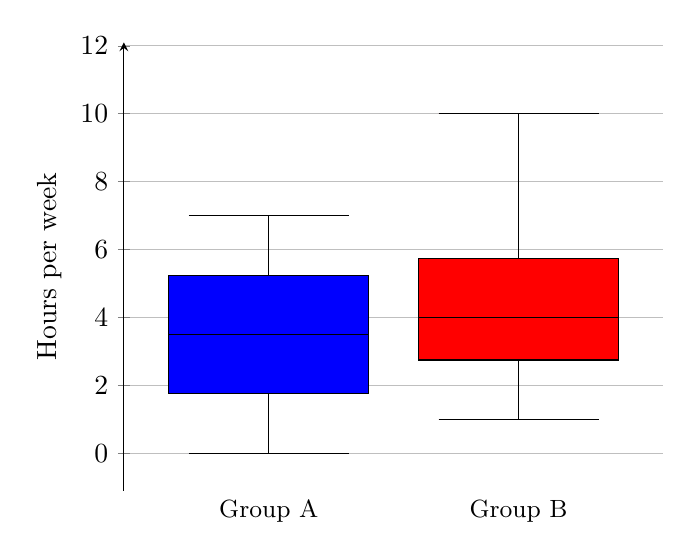
\begin{tikzpicture}
  % --- raw data ---------------------------------------------------------------
  % Each row is one group; PGFPlots will transpose so that every *column*
  % becomes a separate box plot.
  \begin{filecontents*}{twogroups.csv}
  1,2,3,4,4,5,8,10   % Group A (right-skewed)
  1,2,3,4,4,5,6,7    % Group B (roughly symmetric)
  \end{filecontents*}

  % --- PGFPlots set-up --------------------------------------------------------
  \pgfplotstableread[col sep=comma]{twogroups.csv}\csvdata
  \pgfplotstabletranspose\datatransposed{\csvdata}   % rows → columns

  \begin{axis}[
      boxplot/draw direction         = y,
      x axis line style              = {opacity=0},
      axis x line*                   = bottom,
      axis y line                    = left,
      enlarge y limits,
      ymajorgrids,
      ymin                            = 0,
      ymax                            = 11,
      ylabel                          = {Hours per week},
      xtick                           = {1,2},
      xticklabels                     = {Group A, Group B},
      xticklabel style                = {align=center, font=\small},
      xtick style                     = {draw=none},  % hide tick line
  ]
      % Two box plots: columns 0 and 1 of the transposed table
      \foreach \n in {0,1}{
          \addplot+[
              boxplot,
              fill,
              draw=black,
          ]
          table[y index=\n] {\datatransposed};
      }
  \end{axis}
\end{tikzpicture}
\end{center}

\begin{itemize}
  \item Compare the two distributions in terms of \emph{shape, center, and spread}.  
        Note in particular that both groups have the same median (4 hours) but
        Group A shows a much longer right tail, indicating greater variability
        and positive skewness.
\end{itemize}
% ----------------------------------------------------------------------------- 
